\documentclass{article}
\usepackage{graphicx}
\usepackage{amsmath}
\usepackage{gensymb}

\author{Timothy Boose\\Reed Fowler\\Justin Joy\\Dylan Orozco\bigskip\\Physics 188}
\date{\today}
\title{Lab 7 Report - Group 7}

\begin{document}
\maketitle

\section{Goal}

The goal of this lab was to do the following:

\begin{itemize}
    \item Measure the orbital velocity of matter in the Milky Way
    \item Measure the mass of the Milky Way that resides within certain radii
    \item Determine whether the mass of the Milky Way is concentrated predominately within its center or whether this mass is spread out throughout the galaxy's disk
    \item Determine whether the Milky Way is predominately composed of visible or dark matter
\end{itemize}

\section{Skills Learned}

We learned the following skills during this exercise:

\begin{itemize}
    \item How to use Skynet to take radio observations using Green Bank Observatory's radio telescope
    \item How to use the data from these radio observations to determine both the orbital velocity of regions of the Milky Way as well as the distance of these regions from the center of the Milky Way
    \item How to plot the velocity of regions of the Milky Way against their distance from the center of the Milky Way, as well as how to use this plot to determine where the mass of the Milky Way is concentrated
    \item How to determine the mass of objects in the Milky Way that orbit below a certain radius
    \item How to use the orbital velocity of and distance from the center of the Milky Way of the Large and Small Magellanic Clouds to determine whether Dark or Visible matter is more prevalent in the Milky Way
\end{itemize}

\section{Data Collected}

The following data was collected:

\begin{itemize}
    \item e
\end{itemize}

The following data was provided and used in our analysis:

\begin{itemize}
    \item 
\end{itemize}

\section{Analysis of Data}

\section{Figures}
\begin{center}
    \begin{figure}[h!bt]
        \caption{
            e
            \smallskip
        }
        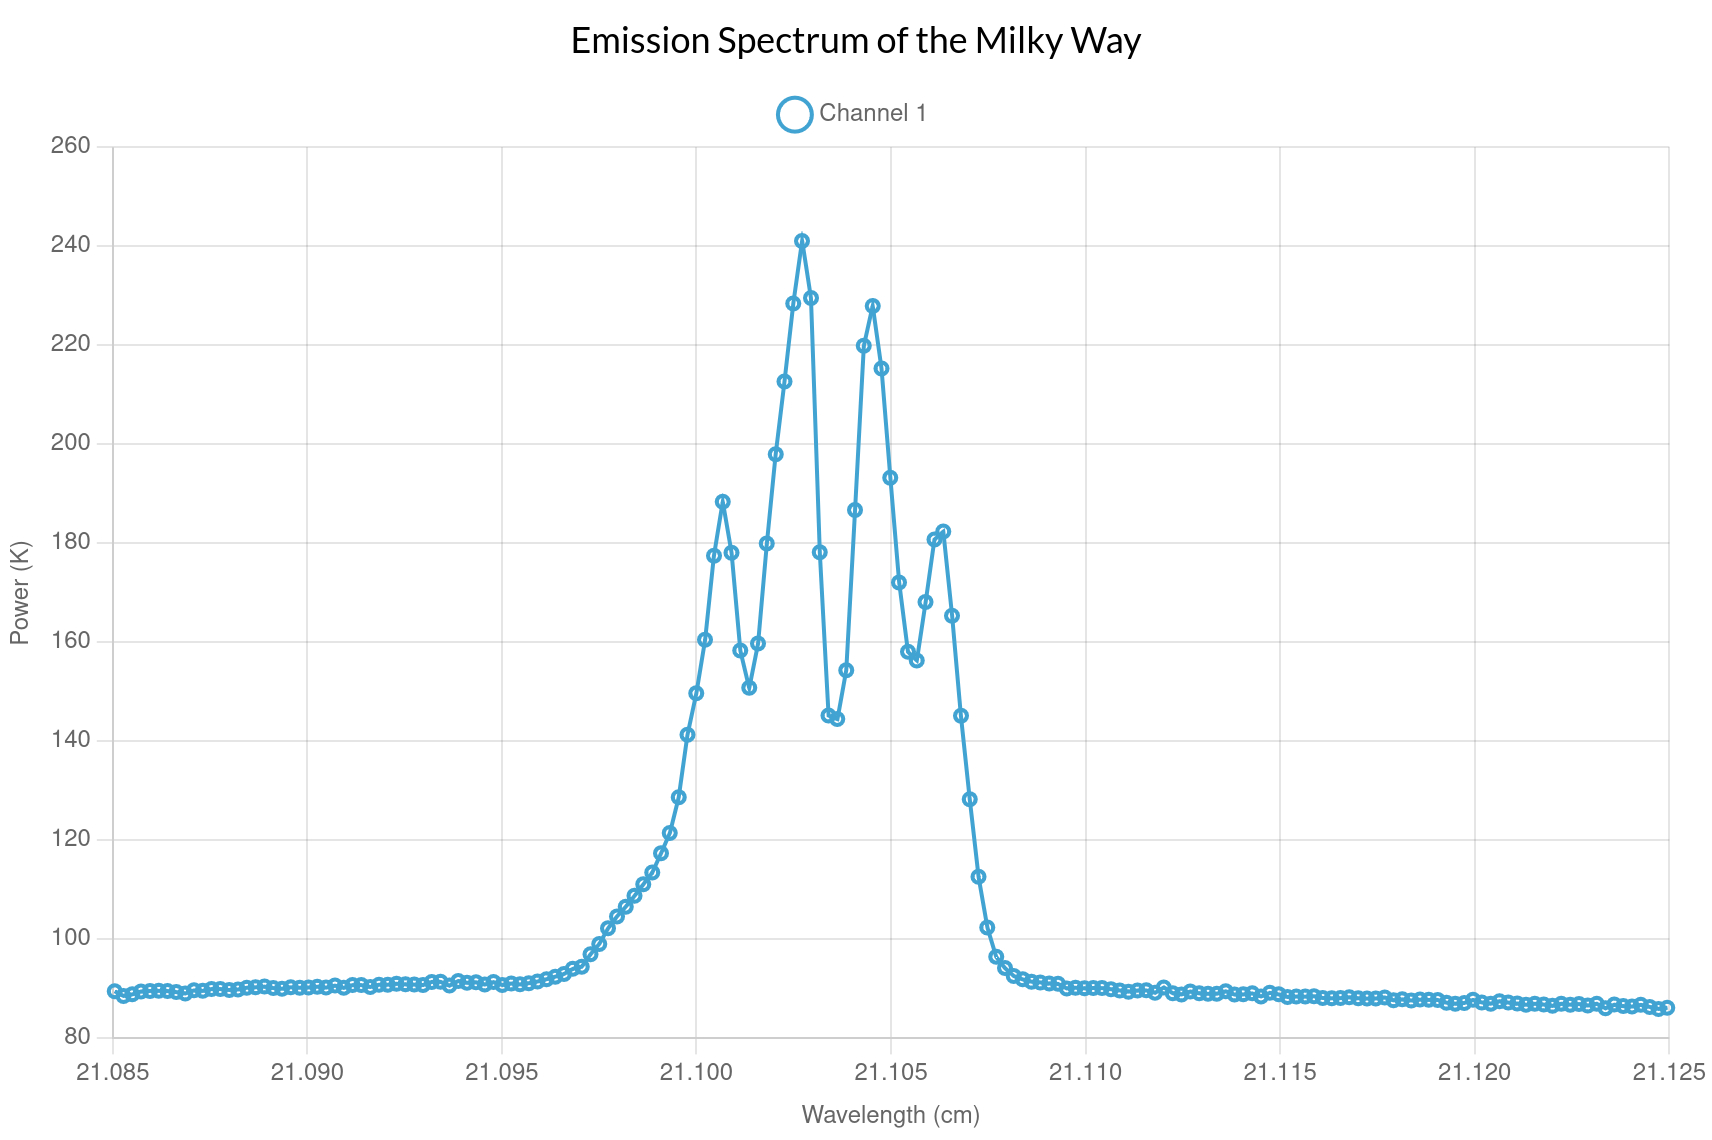
\includegraphics[scale=0.1]{emission-graph-lab9.jpg}
        \centering
    \end{figure}
    \begin{figure}[h!bt]
        \caption{
            e
            \smallskip
        }
        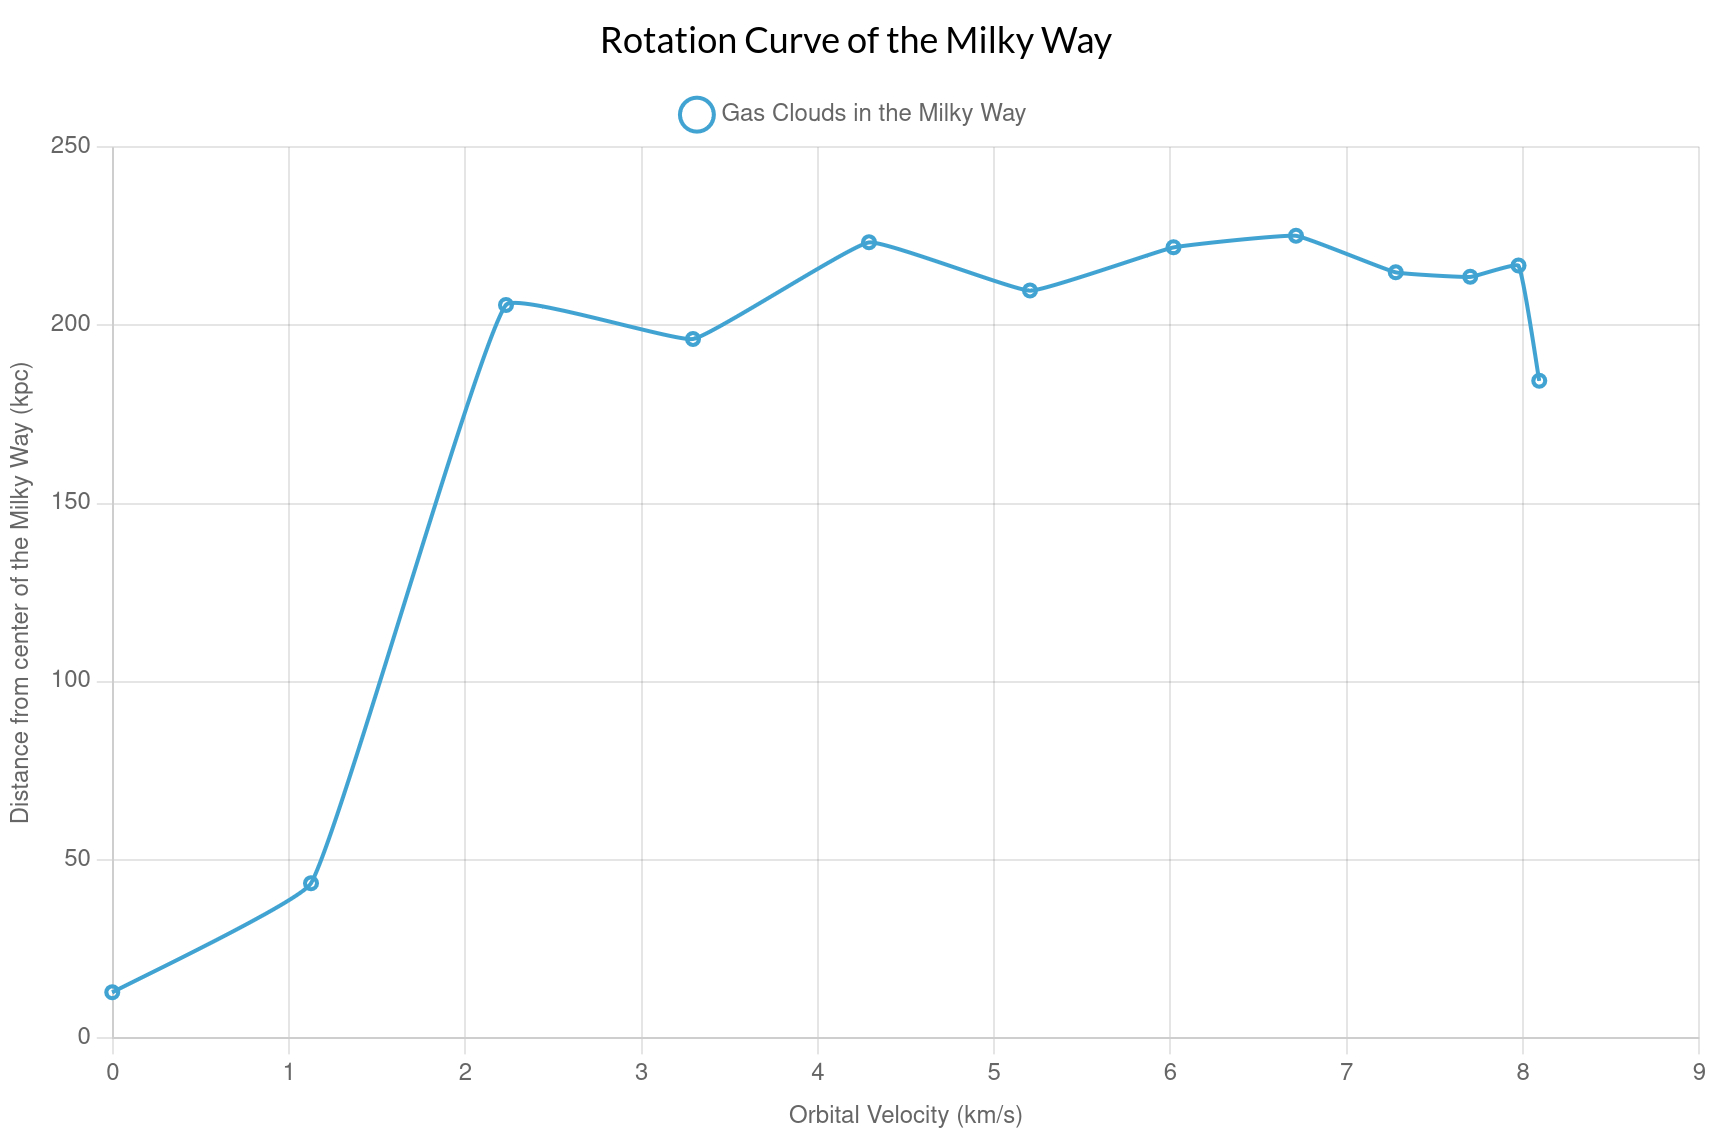
\includegraphics[scale=0.1]{rotation-curve-lab9.jpg}
        \centering
    \end{figure}
    \begin{figure}[h!bt]
        \caption{
            e
            \smallskip
        }
        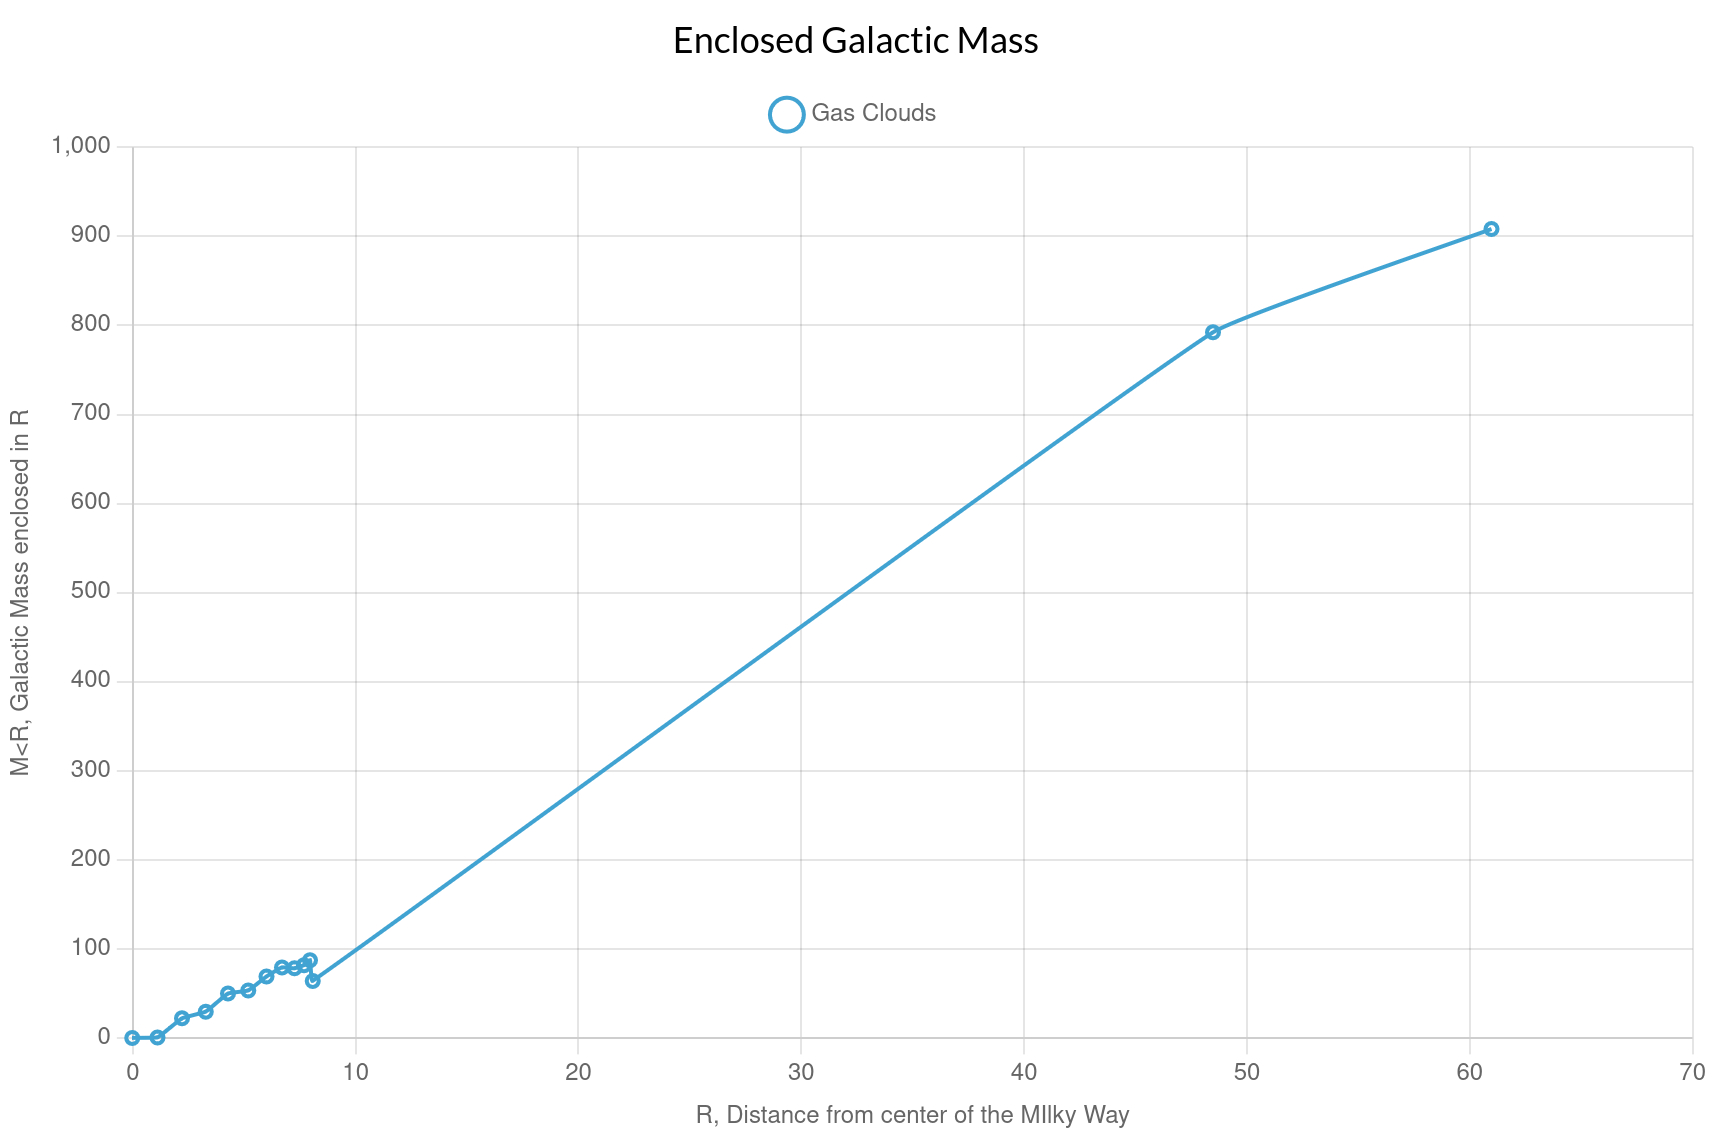
\includegraphics[scale=0.1]{distance-enclosed-mass.jpg}
        \centering
    \end{figure}
\end{center}

\section{Conclusion}



\section{Limitations}



\subsection{Errors}



\subsection{Impact of Errors}



\end{document}